\documentclass{article}
\usepackage{tikz}
\usepackage{caption}
\usepackage{listings}
\usepackage{xcolor}
\usepackage{multicol}
\usepackage{geometry}
\usepackage{hyperref}
\lstset { %
    language=Python,
    backgroundcolor=\color{black!5}, % set backgroundcolor
    basicstyle=\footnotesize,% basic font setting
}
\usetikzlibrary{shapes}
\geometry{
  left={1cm},
  right={1cm}
}

\author{Asher Griess, David Medin}
\title{R Tree Algorithm}
\begin{document}
\maketitle
\begin{center}
Github URL : \url{https://github.com/asherkendall/r-tree-implementation}
\end{center}

\begin{multicols}{2}[]
\section{Abstract}
\paragraph{}
An R Tree is a data structure used to perform spacial computations and comparisons much faster than using a brute force algorithm.
The R tree is very similar to the B-tree in structure, and Quad-Tree in use. One of the main differences is that
R trees are page-able. This means that they could be put into storage, which is ideal when working with very large data sets 
that cannot be stored in RAM. It is also possible to move segments of the R tree into RAM while working with it. Additionally, it is not limited to representing only one dimension as with B Trees, but up to $N$ dimensions. A good example
of a program that is well-suited to the use of R-trees is that of a mapping system of the world, where the large data set would be hard to store in memory.
The R tree is very applicable for conducting a nearest neighbor search, and storing any type of shape which allow for shapes
of things, such as buildings, to be put in the minimum bounding rectangle. R trees are commonly used in databases to represent spacial data.
Spliting is one the most expensive parts of the R-tree, which makes it suitable for data that doesn't change often.

\section{Basics}

\paragraph{}
An R Tree is parameterized by two variables, $M$, which specifies the maximum number of entries each node is allowed to have, and
 the number of dimensions of the space the R Tree is mapping. An entry of a node is either a reference
to another node, or a data object. In this implementation, all data objects are points in space, but it is also possible to have any combination
 of shapes in a R Tree so long as equality can be tested, and the minimum bounding rectangle can be calculated.
Based on $M$, is $m = \lceil\frac{M}{2}\rceil$, which is the minimum number of entries each node must have. A reasonable value for $M$ is 50.
 \cite{guttman_1984_rtrees} Each entry of a node must have an Minimum Bounding Rectangle,
or MBR (which also serves as an AABB). This is a bounding rectangle that tightly encloses all of its contents. If an entry to a node is another node
which are all parents, then the entry of the first node will have an MBR encompassing all of its child nodes.
Similarly, entries that point to leaf nodes have an MBR encompassing all of the data objects - or points - that belong to that leaf node.

\section{Inserting}
\paragraph{}
There is no average complexity for an R Tree, but the worst possible
case is of complexity $O(n)$. This is because it is possible that every node will have to be searched, all $n$ nodes. If root is a leaf node, then add it to root without question. If this would cause any node to have
 more than $M$ entries, then it is necessary to split the node. If the node has children, then locate any node which can wholly
fit the object, or the node who's MBR's area will change the least if it were added to the node.  This process is continued down the tree until reaching a leaf node that either is able to contain the object or will change the area by an insignificant amount. Lastly, insert. If the number of entries of the leaf node exceeds $M$, then it is necessary to split the node.

\begin{minipage}{\linewidth}
\captionof{figure}{R-Tree Example}
\centering
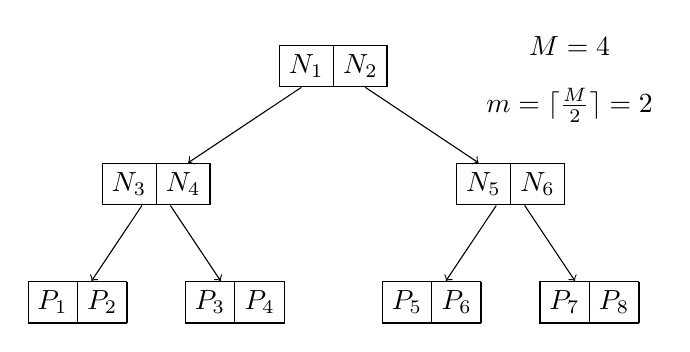
\begin{tikzpicture}
  \draw (3cm,0.25cm) node{$M = 4$};
  \draw (3cm,-0.5cm) node{$m= \lceil\frac{M}{2}\rceil = 2$};
  \tikzstyle{rtree}=[rectangle split, rectangle split horizontal,rectangle split ignore empty parts,draw]
  \tikzstyle{every node}=[rtree]
  \tikzstyle{level 1}=[sibling distance=45mm]
  \tikzstyle{level 2}=[sibling distance=20mm]
  \node {$N_1$ \nodepart{two} $N_2$} [->]
      child {node {$N_3$ \nodepart{two} $N_4$}
      child {node {$P_1$ \nodepart{two} $P_2$}}
      child {node {$P_3$ \nodepart{two} $P_4$}}    
  } 
  child {node {$N_5$ \nodepart{two} $N_6$}
      child {node {$P_5$ \nodepart{two} $P_6$}}
      child {node {$P_7$ \nodepart{two} $P_8$}} 
};
\end{tikzpicture}

Note: In this example the leaf nodes contain the actual points or shapes($P_n$).
\end{minipage}

% \subsection*{Pseudo Code}
% This process is shown as pseudo code below


% \begin{lstlisting}
% Insert(node, object)
%   best_node = null
%   min_area_change = inf
%   for entry in node.entries:
%     if entry.can_hold(object):
%       Insert(entry)
%       break
    
% % If at leaf:
% %   Insert(Entry)
% %   If(entries > M):
% %     Split()
% %   CurrentNode.entries.Add(Entry)
% %   return
% % For(each child):
% %   If(ChildNode.IsEngulf(Entry)):
% %     Insert(Node)
% %   else:
% %     For(each child):
% %       Find difference in area if Entry were inserted
% %     insert(NodeWithSmallestDifference);
% \end{lstlisting}


\section{Splitting} 

\paragraph{}
When performing a split, the goal is to take a node that has too many entries and split it into
two nodes that contain at least $m$ entries, and reduce the total area of each nodes' MBR as much as possible. This implementation utilizes a Linear Split, but there are other
algorithms such as quadratic split and exhaustive split, the later of which checks every
possible split and chooses the option with the least area. An Exhaustive Split
will not make any "bad" splits. The Linear Split algorithm
is linear in $M$ and the number of dimensions of the space. It often does sub-optimal
splits, but it is much better than the exhaustive split complexity of $O(d^{M-1})$, where
$d$ is the number of dimensions. This is because for each dimension, we need to compare every
entry, up to $M+1$, with each other entry.

\paragraph{}
The first step in the linear split algorithm is to find the two entries that will be the
start of the two new nodes produced from this split. The two starting entries will be the
entries with the greatest difference in a dimension. Firstly, compare the $x$'s, then the $y$'s,
and so on for however many dimensions the R Tree has. One of the starting entries is inserted into node one,
the other into node two. Then, for all other entries, test which MBR of the two nodes' area
will change the least if it expands to encompass the entry, and add that entry to said node. Do this
until either all entries are split between the two nodes or one of the nodes must claim the
rest of the entries in order to have at least $m$ entries. Lastly, set the parent of the two
new nodes to the parent of the old node, and delete the old node. Keep in mind that one may have to
recurse up the tree adjusting all connected nodes.
\section{Searching}
\paragraph{}
To search an R Tree an object is given to the structure, and the R Tree will recurse itself for
an object that is equal to the desired object and return the node that contains it. Searching an R Tree has an average complexity
of $O(log_Mn)$, and a worst case of $O(n)$, making it better, on average, as $M$ increases, the maximum number of entries
per node. Searching can result in searching through every node, which is $n$, but the effort could be divided by $M$, the
number of entries a node can have.
\paragraph{}
Firstly, the MBR of the root node is checked to see whether it contains the object. If it doesn't, then it is impossible for it to be contained by any of its children and the search ends.
If it is contained, then each child is checked to see whether the object is totally contained.
For each child that does contain the object, we'll recurse down and start the process over again until we reach a leaf node that
is able to wholly contain the object's MBR inside its MBR. Then, we compare each leaf node entry with the object. If any are equal, then
return the found the leaf node and the search is concluded.

\section{Removing}

\paragraph{}
When removing a point - or an object - from a R Tree, the first step is to find the leaf node that stores the point.
This process is covered in the previous section, Searching. After identifying the leaf node that contains
the point, the next step is to remove the point from the leaf node. This may reduce the number of entries this leaf node has to be below
$m$, which is not allowed for nodes that are not root. If the leaf node is the root then this is issue is ignored, as it is not possible to have a smaller tree.\\

\begin{minipage}{\linewidth}
\captionof{figure}{A snapshot of the bottom of an R Tree. $N_{parent}$\\ represents the rest of the tree, and $P_n$ represents the data\\ objects.}
\centering
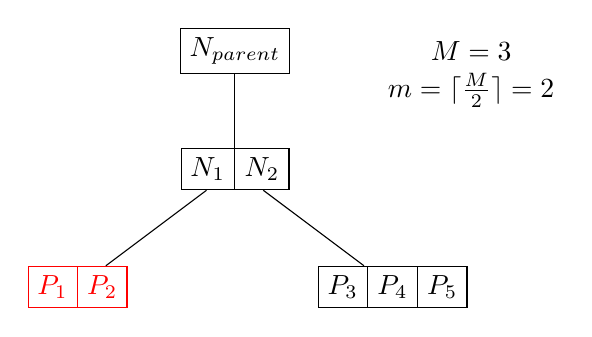
\begin{tikzpicture}
  \draw (3cm,0) node{$M=3$};
  \draw (3cm,-0.5cm) node{$m= \lceil\frac{M}{2}\rceil = 2$};
  \tikzstyle{rtree}=[rectangle split, rectangle split horizontal,rectangle split ignore empty parts,draw]
    \tikzstyle{every node}=[rtree]
    \tikzstyle{level 1}=[sibling distance=45mm]
    \tikzstyle{level 2}=[sibling distance=40mm]
    \node{$N_{parent}$}
    child {node{$N_1$ \nodepart{two} $N_2$}
      child{node[color=red]{$P_1$ \nodepart{two} $P_2$} }
      child{node{$P_3$ \nodepart{two} $P_4$ \nodepart{three} $P_5$}}
    };
\end{tikzpicture}
\label{fig:removing}
\end{minipage}

\paragraph{}
In Figure \ref{fig:removing}, the leaf node $N_1$, which has two entries, is going to have an entry removed.
 Because $m=3$, the red leaf node will be deleted and its other entry will be reinserted later. After this operation, because $N_{parent}$
 contains only one entry, it will be deleted, and it's children will be recursed to find the three entries in $N_2$ and store those for reinsertion as well.
\paragraph{}
If this node is not the root and has less than $m$ entries, then it is necessary to delete that node. But the other $m - 1$ entries should not be destroyed, so each of the node's entries will be stored into a list, or other container type, to insert back into
the tree when the removal operation concludes. Because the leaf node is being removed, this means that its parent's entries can also fall below
$m$ nodes, which then requires that it is deleted too. In that case, a recursive search of all of that parent's children is necessary
to find all points - or other data objects - to store for reinsertion later.
\paragraph{}
Even though it seems that a the leaf node case and the parent node case seem different, they are actually the same case. Parents have
other nodes as their entries and leaf nodes have objects as their entries. Both must have $m \le n \le M$ entries (where $n$ is the number
of entries the node has), and both need to be deleted from their parent and recursively store all of the entries below it in the tree.
Unfortunately, it was not possible to identify a complexity for removing, but it would be very significant. Not only does the algorithm search, it might also
need to remove $1/M$ of the tree, and then reinsert them all.
\bibliographystyle{plain}
\bibliography{rtree.bib}

\end{multicols}

\end{document}